%%%%%%%%%%%%%%%%%%%%%%%%%%%%%%%%%%%%

\section{重回帰入門}

%%%%%%%%%%%%%%%%%%%%%%%%%%%%%%%%%%%%

\begin{frame}
\frametitle{重回帰}

\begin{itemize}

\item 単純線形回帰：2変数 --- 応答変数 $y$ と説明変数 $x$

\item 重線形回帰：複数変数 --- 応答変数 $y$ と説明変数 $x_1, x_2, \cdots$

\end{itemize}

\end{frame}

%%%%%%%%%%%%%%%%%%%%%%%%%%%%%%%%%%%%

\subsection{ダミー変数とカテゴリ変数を予測変数として用いる}

%%%%%%%%%%%%%%%%%%%%%%%%%%%%%%%%%%%

\begin{frame}
\frametitle{貧困率 vs. 地域（東部・西部）}


\[ \widehat{poverty} = 11.17 + 0.38 \times west \]

\begin{itemize}

\item 説明変数：地域、\hl{参照水準：}東部（east）

\item \hl{切片：}東部の州における貧困率の推定平均は 11.17\%
\begin{itemize}
\item 説明変数に \orange{0} を代入したときの値
\end{itemize}

\item \hl{傾き：}西部の州における貧困率の推定平均は東部より 0.38\% 高い。
\begin{itemize}
\item したがって、西部の州の貧困率の推定平均は 11.17 + 0.38 = 11.55\%。
\item 説明変数に \orange{1} を代入したときの値
\end{itemize}

\end{itemize}

\end{frame}

%%%%%%%%%%%%%%%%%%%%%%%%%%%%%%%%%%

\begin{frame}
\frametitle{貧困率 vs. 地域（北東部・中西部・西部・南部）}

\pq{北東部（northeast）・中西部（midwest）・西部（west）・南部（south）のうち、参照水準はどれか？}

{\small
\begin{center}
\begin{tabular}{rrrrr}
  \hline
 & Estimate & Std. Error & t value & Pr($>$$|$t$|$) \\
  \hline
(Intercept) & 9.50 & 0.87 & 10.94 & 0.00 \\
region4midwest & 0.03 & 1.15 & 0.02 & 0.98 \\
region4west & 1.79 & 1.13 & 1.59 & 0.12 \\
region4south & 4.16 & 1.07 & 3.87 & 0.00 \\
   \hline
\end{tabular}
\end{center}
}

\begin{enumerate}[(a)]
\solnMult{northeast（北東部）}
\item midwest（中西部）
\item west（西部）
\item south（南部）
\item 判別できない
\end{enumerate}

\end{frame}

%%%%%%%%%%%%%%%%%%%%%%%%%%%%%%%%%%%

\begin{frame}
\frametitle{貧困率 vs. 地域（北東部・中西部・西部・南部）}

\pq{北東部・中西部・西部・南部のうち、最も貧困率が低い地域はどれか？}

{\small
\begin{center}
\begin{tabular}{rrrrr}
  \hline
 & Estimate & Std. Error & t value & Pr($>$$|$t$|$) \\
  \hline
(Intercept) & 9.50 & 0.87 & 10.94 & 0.00 \\
region4midwest & 0.03 & 1.15 & 0.02 & 0.98 \\
region4west & 1.79 & 1.13 & 1.59 & 0.12 \\
region4south & 4.16 & 1.07 & 3.87 & 0.00 \\
   \hline
\end{tabular}
\end{center}
}

\begin{enumerate}[(a)]
\solnMult{northeast（北東部）}
\item midwest（中西部）
\item west（西部）
\item south（南部）
\item 判別できない
\end{enumerate}

\end{frame}

%%%%%%%%%%%%%%%%%%%%%%%%%%%%%%%%%%%%

\subsection{モデルへの多変数の組み込みと評価}

%%%%%%%%%%%%%%%%%%%%%%%%%%%%%%%%%%%%

\begin{frame}
\frametitle{本の重量}

\twocol{0.6}{0.4}{
{\footnotesize
\begin{center}
\begin{tabular}{rrrc}
  \hline
 & 重量 (g) & 体積 (cm$^\text{3}$) & カバー \\
  \hline
1 & 800 & 885 & hc \\
  2 & 950 & 1016 & hc \\
  3 & 1050 & 1125 & hc \\
  4 & 350 & 239 & hc \\
  5 & 750 & 701 & hc \\
  6 & 600 & 641 & hc \\
  7 & 1075 & 1228 & hc \\
  8 & 250 & 412 & pb \\
  9 & 700 & 953 & pb \\
  10 & 650 & 929 & pb \\
  11 & 975 & 1492 & pb \\
  12 & 350 & 419 & pb \\
  13 & 950 & 1010 & pb \\
  14 & 425 & 595 & pb \\
  15 & 725 & 1034 & pb \\
   \hline
\end{tabular}
\end{center}
}}
{
\begin{center}
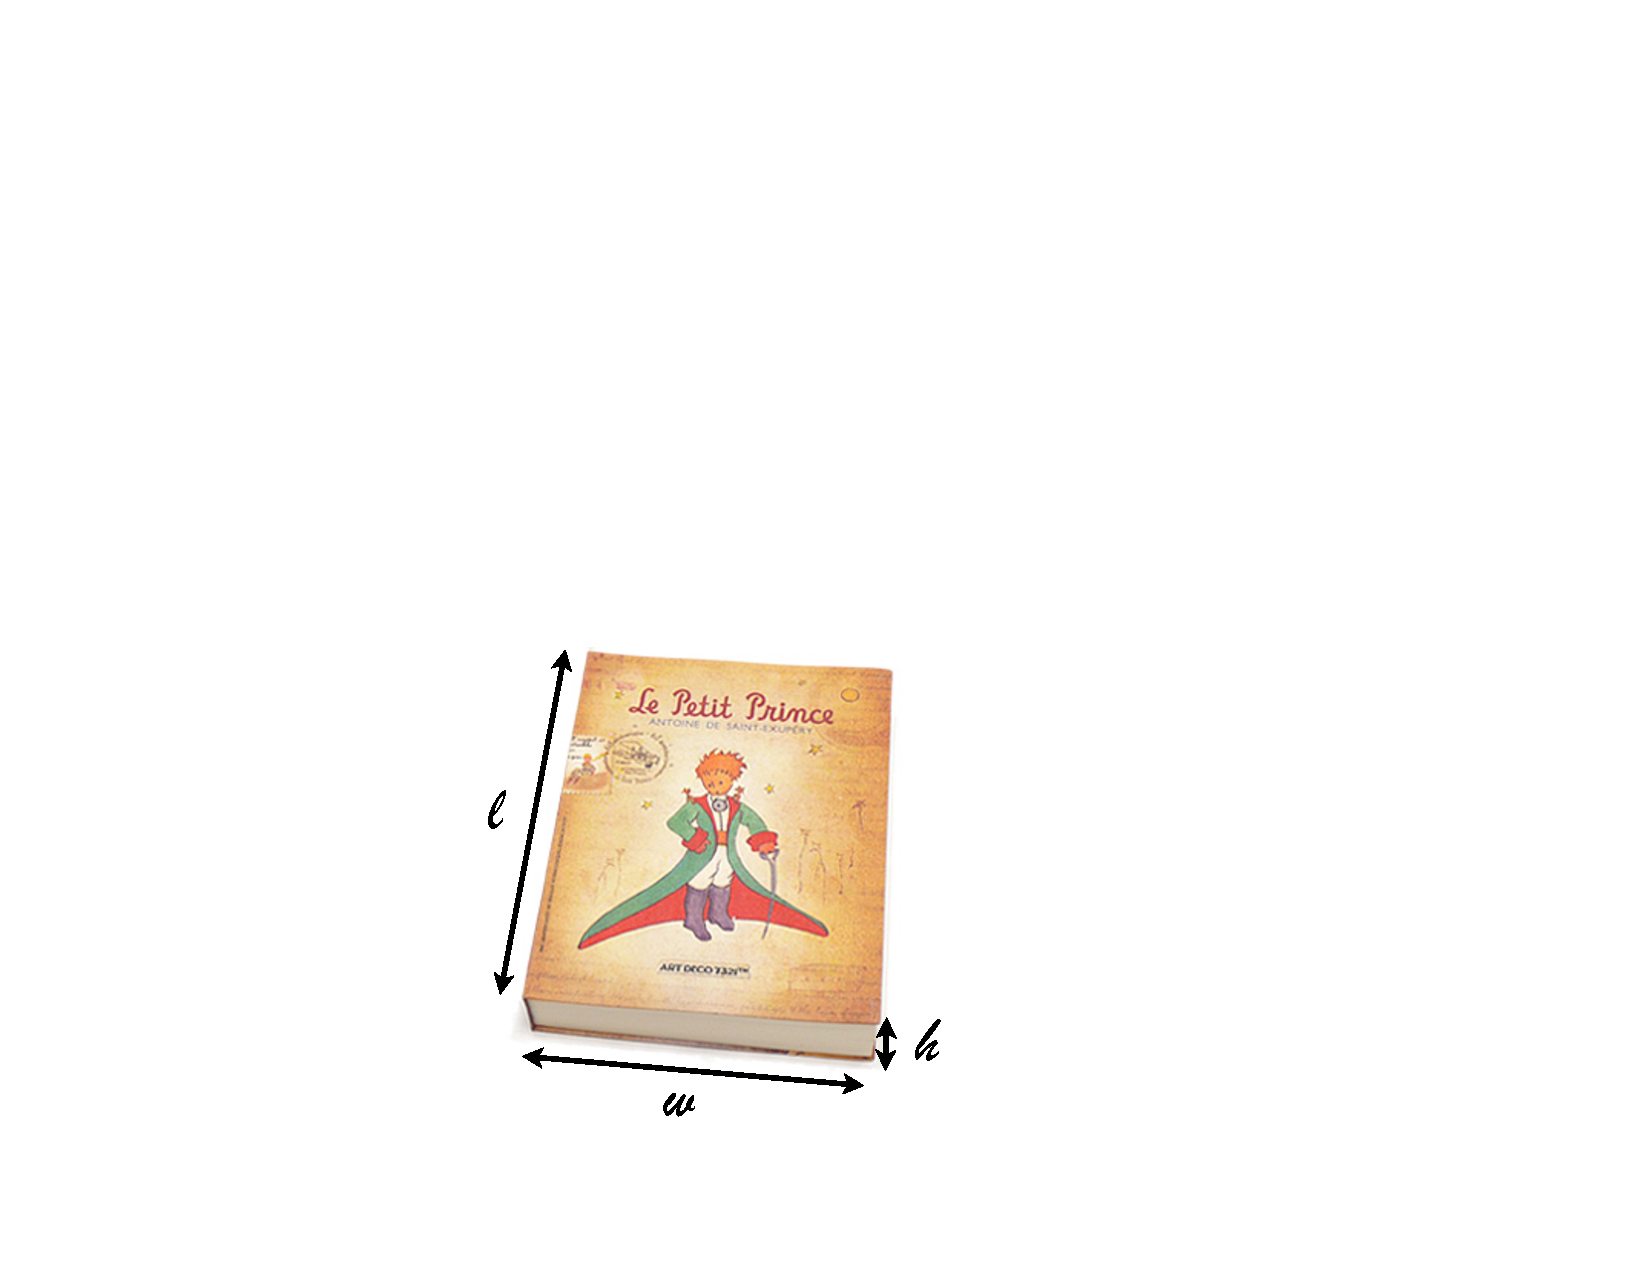
\includegraphics[width=0.7\textwidth]{9-1_intro_mlr/figures/books/book}
\end{center}
}

\ct{From: Maindonald, J.H. and Braun, W.J. (2nd ed., 2007) ``Data Analysis and Graphics Using R"}

\end{frame}

%%%%%%%%%%%%%%%%%%%%%%%%%%%%%%%%%%%

\begin{frame}
\frametitle{本の重量（続き）}

\twocol{0.45}{0.4}
{
\pq{{\small 散布図は本の重量と体積の関係、および回帰出力を示している。以下のうち正しいものはどれか？}}
}
{
\begin{center}
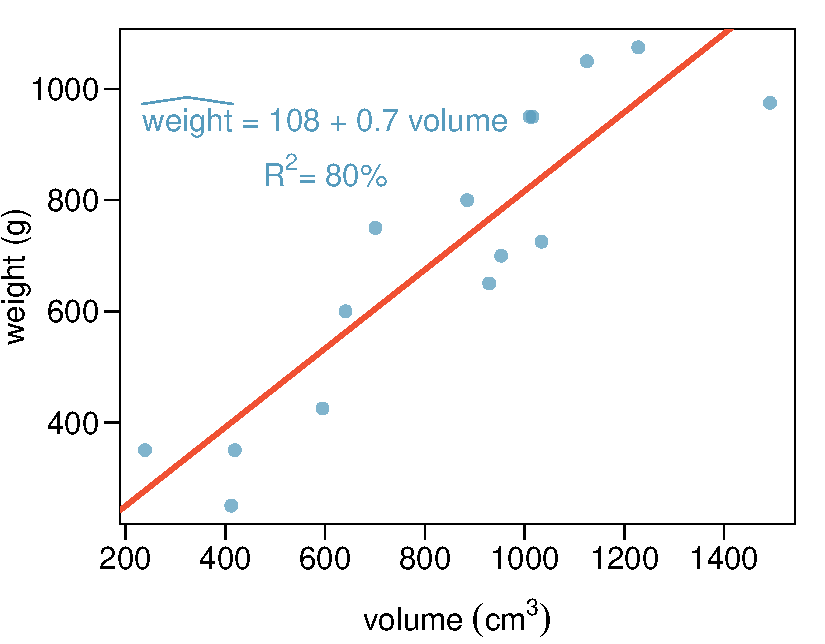
\includegraphics[width=\textwidth]{9-1_intro_mlr/figures/books/weight_volume}
\end{center}
}

\begin{enumerate}[(a)]
\item このモデルで本の 80\% の重量を正確に予測できる。
\solnMult{体積が平均より 10 cm$^\text{3}$ 大きい本は、重量が平均より約 7 g 重いと予測される。}
\item 重量と体積の相関係数は $R = 0.80^2 = 0.64$ である。
\item このモデルは最も体積の大きい本の重量を過小推定している。
\end{enumerate}

\end{frame}

%%%%%%%%%%%%%%%%%%%%%%%%%%%%%%%%%%%

\begin{frame}[fragile]
\frametitle{体積を用いた本の重量のモデリング}

{\small \textit{出力の一部を省略...}}

\begin{verbatim}
Coefficients:
             Estimate Std. Error t value Pr(>|t|)
(Intercept) 107.67931   88.37758   1.218    0.245
volume        0.70864    0.09746   7.271 6.26e-06


Residual standard error: 123.9 on 13 degrees of freedom
Multiple R-squared: 0.8026,	Adjusted R-squared: 0.7875
F-statistic: 52.87 on 1 and 13 DF,  p-value: 6.262e-06
\end{verbatim}

\end{frame}

%%%%%%%%%%%%%%%%%%%%%%%%%%%%%%%%%%%

\begin{frame}
\frametitle{ハードカバーとペーパーバックの重量}

\dq{ハードカバーとペーパーバックの体積と重量の関係において、何かトレンドを見つけられるか？}

\soln{{\small 体積を一定にした場合、ペーパーバックは一般的にハードカバーより軽い。}}

\begin{center}
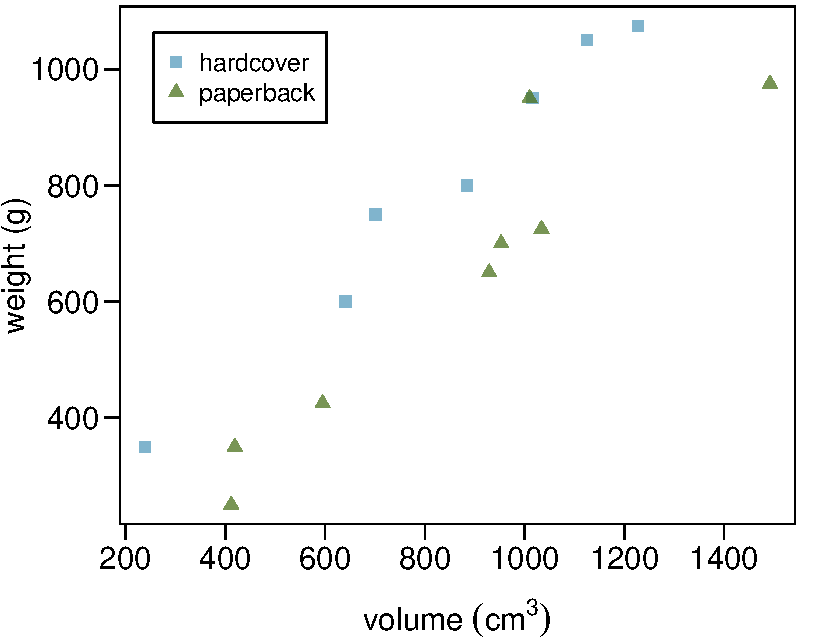
\includegraphics[width=0.6\textwidth]{9-1_intro_mlr/figures/books/weight_volume_cover}
\end{center}

\end{frame}

%%%%%%%%%%%%%%%%%%%%%%%%%%%%%%%%%%%

\begin{frame}[fragile]
\frametitle{体積\underline{とカバー種類}を用いた本の重量のモデリング}

\begin{verbatim}
Coefficients:
              Estimate Std. Error t value Pr(>|t|)
(Intercept)  197.96284   59.19274   3.344 0.005841 **
volume         0.71795    0.06153  11.669  6.6e-08 ***
cover:pb    -184.04727   40.49420  -4.545 0.000672 ***


Residual standard error: 78.2 on 12 degrees of freedom
Multiple R-squared: 0.9275,	Adjusted R-squared: 0.9154
F-statistic: 76.73 on 2 and 12 DF,  p-value: 1.455e-07
\end{verbatim}

\end{frame}

%%%%%%%%%%%%%%%%%%%%%%%%%%%%%%%%%%%

\begin{frame}
\frametitle{参照水準の決定}

\pq{以下の回帰出力に基づき、変数 \var{cover} の参照水準はどれか？なお \var{pb}：ペーパーバック。}

{\small
\begin{center}
\begin{tabular}{rrrrr}
  \hline
 & Estimate & Std. Error & t value & Pr($>$$|$t$|$) \\
  \hline
(Intercept) & 197.9628 & 59.1927 & 3.34 & 0.0058 \\
  volume & 0.7180 & 0.0615 & 11.67 & 0.0000 \\
  cover:pb & -184.0473 & 40.4942 & -4.55 & 0.0007 \\
   \hline
\end{tabular}
\end{center}
}

\begin{enumerate}[(a)]
\item ペーパーバック（paperback）
\solnMult{ハードカバー（hardcover）}
\end{enumerate}

\end{frame}

%%%%%%%%%%%%%%%%%%%%%%%%%%%%%%%%%%%

\begin{frame}
\frametitle{参照水準の決定}

\pq{以下のうち、この回帰モデルにおける変数の役割を正しく説明しているものはどれか？}

{\small
\begin{center}
\begin{tabular}{rrrrr}
  \hline
 & Estimate & Std. Error & t value & Pr($>$$|$t$|$) \\
  \hline
(Intercept) & 197.9628 & 59.1927 & 3.34 & 0.0058 \\
  volume & 0.7180 & 0.0615 & 11.67 & 0.0000 \\
  cover:pb & -184.0473 & 40.4942 & -4.55 & 0.0007 \\
   \hline
\end{tabular}
\end{center}
}

\begin{enumerate}[(a)]
\item 応答変数：重量、説明変数：体積、ペーパーバック
\item 応答変数：重量、説明変数：体積、ハードカバー
\item 応答変数：体積、説明変数：重量、カバー種類
\solnMult{応答変数：重量、説明変数：体積、カバー種類}
\end{enumerate}

\end{frame}

%%%%%%%%%%%%%%%%%%%%%%%%%%%%%%%%%%%

\begin{frame}
\frametitle{線形モデル}

{\small
\begin{center}
\begin{tabular}{rrrrr}
  \hline
 & Estimate & Std. Error & t value & Pr($>$$|$t$|$) \\
  \hline
(Intercept) & 197.96 & 59.19 & 3.34 & 0.01 \\
  volume & 0.72 & 0.06 & 11.67 & 0.00 \\
  cover:pb & -184.05 & 40.49 & -4.55 & 0.00 \\
   \hline
\end{tabular}
\end{center}
}

\[ \widehat{weight} = 197.96 + 0.72~volume - 184.05~cover:pb  \]

\begin{enumerate}

\item \hl{ハードカバー}の場合：\var{cover} に \orange{0} を代入
\begin{eqnarray*}
\widehat{weight} &=& 197.96 + 0.72~volume - 184.05 \times \orange{0} \\
&=& 197.96 +  0.72~volume
\end{eqnarray*}

\item \orange{ペーパーバック}の場合：\var{cover} に \orange{1} を代入
\begin{eqnarray*}
\widehat{weight} &=& 197.96 + 0.72~volume - 184.05 \times \orange{1} \\
&=& 13.91 +  0.72~volume
\end{eqnarray*}

\end{enumerate}

\end{frame}

%%%%%%%%%%%%%%%%%%%%%%%%%%%%%%%%%%%

\begin{frame}
\frametitle{線形モデルの可視化}

\begin{center}
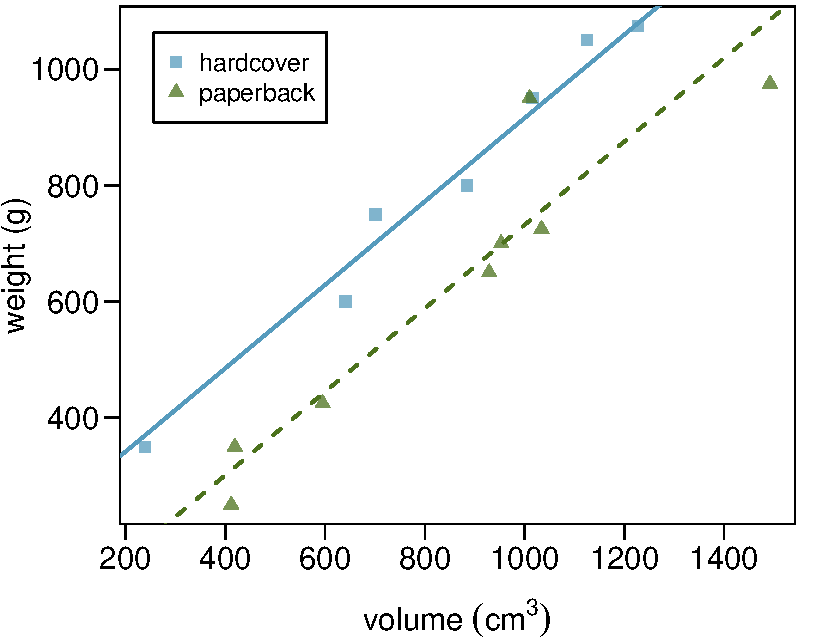
\includegraphics[width=0.8\textwidth]{9-1_intro_mlr/figures/books/weight_volume_cover_lines}
\end{center}

\end{frame}

%%%%%%%%%%%%%%%%%%%%%%%%%%%%%%%%%%%

\begin{frame}
\frametitle{回帰係数の解釈}

{\small
\begin{center}
\begin{tabular}{rrrrr}
  \hline
 & Estimate & Std. Error & t value & Pr($>$$|$t$|$) \\
  \hline
(Intercept) & 197.96 & 59.19 & 3.34 & 0.01 \\
  volume & 0.72 & 0.06 & 11.67 & 0.00 \\
  cover:pb & -184.05 & 40.49 & -4.55 & 0.00 \\
   \hline
\end{tabular}
\end{center}
}

\begin{itemize}

\item \hl{体積の傾き：}\underline{他の変数を一定に保つと}、体積が 1 cm$^3$ 大きい本は重量が約 0.72 g 重い傾向がある。

\item \hl{カバーの傾き：}\underline{他の変数を一定に保つと}、ペーパーバックはハードカバーより 184 g 軽いとモデルは予測する。

\item \hl{切片：}体積ゼロのハードカバーの平均重量は 198 g と予測される。
\begin{itemize}
\item 明らかに、この切片は文脈的に意味をなさない。直線の高さを調整するためだけのものである。
\end{itemize}

\end{itemize}

\end{frame}

%%%%%%%%%%%%%%%%%%%%%%%%%%%%%%%%%%%

\begin{frame}
\frametitle{予測}

\pq{体積が 600 cm$^3$ のペーパーバックの予測重量を求める正しい計算式はどれか？}

{\small
\begin{center}
\begin{tabular}{rrrrr}
  \hline
 & Estimate & Std. Error & t value & Pr($>$$|$t$|$) \\
  \hline
(Intercept) & 197.96 & 59.19 & 3.34 & 0.01 \\
  volume & 0.72 & 0.06 & 11.67 & 0.00 \\
  cover:pb & -184.05 & 40.49 & -4.55 & 0.00 \\
   \hline
\end{tabular}
\end{center}
}

\begin{enumerate}[(a)]
\solnMult{197.96 + 0.72 * 600 - 184.05 * 1} \only<2->{\orange{~$= 445.91$ グラム}}
\item 184.05 + 0.72 * 600 - 197.96 * 1
\item 197.96 + 0.72 * 600 - 184.05 * 0
\item 197.96 + 0.72 * 1 - 184.05 * 600
\end{enumerate}

\end{frame}

%%%%%%%%%%%%%%%%%%%%%%%%%%%%%%%%%%%

\begin{frame}
\frametitle{別の例：子供の認知テストスコアのモデリング}

3〜4歳の子供の認知テストスコアを母親の特徴で予測する。データは米国成人女性とその子供を対象とした調査（全国縦断的青年調査のサブサンプル）。

{\small
\begin{center}
\begin{tabular}{rrlrlr}
  \hline
 & kid\_score & mom\_hs & mom\_iq & mom\_work & mom\_age \\
  \hline
1 &  65 & yes & 121.12 & yes &  27 \\
  \vdots \\
  5 & 115 & yes & 92.75 & yes &  27 \\
  6 &  98 & no & 107.90 & no &  18 \\
  \vdots \\
  434 &  70 & yes & 91.25 & yes &  25 \\
   \hline
\end{tabular}
\end{center}
}

\vfill

{\tiny Gelman, Hill. \textit{Data Analysis Using Regression and Multilevel/Hierarchical Models}. (2007) Cambridge University Press.}

\end{frame}

%%%%%%%%%%%%%%%%%%%%%%%%%%%%%%%%%%%

\begin{frame}
\frametitle{傾きの解釈}

\dq{\underline{母親の IQ の傾き}の正しい解釈はどれか？}

{\small
\begin{center}
\begin{tabular}{rrrrr}
  \hline
 & Estimate & Std. Error & t value & Pr($>$$|$t$|$) \\
  \hline
(Intercept) & 19.59 & 9.22 & 2.13 & 0.03 \\
  mom\_hs:yes & 5.09 & 2.31 & 2.20 & 0.03 \\
  mom\_iq & 0.56 & 0.06 & 9.26 & 0.00 \\
  mom\_work:yes & 2.54 & 2.35 & 1.08 & 0.28 \\
  mom\_age & 0.22 & 0.33 & 0.66 & 0.51 \\
   \hline
\end{tabular}
\end{center}
}

$\:$ \\

\soln{他の変数を一定に保つと、母親の IQ が 1 点高い子供は平均的に 0.56 点高いスコアをとる傾向がある。}

\end{frame}

%%%%%%%%%%%%%%%%%%%%%%%%%%%%%%%%%%%

\begin{frame}
\frametitle{傾きの解釈}

\dq{\underline{切片}の正しい解釈はどれか？}

{\small
\begin{center}
\begin{tabular}{rrrrr}
  \hline
 & Estimate & Std. Error & t value & Pr($>$$|$t$|$) \\
  \hline
(Intercept) & 19.59 & 9.22 & 2.13 & 0.03 \\
  mom\_hs:yes & 5.09 & 2.31 & 2.20 & 0.03 \\
  mom\_iq & 0.56 & 0.06 & 9.26 & 0.00 \\
  mom\_work:yes & 2.54 & 2.35 & 1.08 & 0.28 \\
  mom\_age & 0.22 & 0.33 & 0.66 & 0.51 \\
   \hline
\end{tabular}
\end{center}
}

$\:$ \\

\soln{高校に行っておらず、子供の生後3年間に働いておらず、IQ が 0 で年齢が 0 歳の母親を持つ子供の平均スコアは 19.59 と推定される。この切片は文脈的に全く意味をなさない。}

\end{frame}

%%%%%%%%%%%%%%%%%%%%%%%%%%%%%%%%%%%

\begin{frame}
\frametitle{傾きの解釈}

\pq{\var{mom\_work} の傾きの正しい解釈はどれか？}

{\scriptsize
\begin{center}
\begin{tabular}{rrrrr}
  \hline
 & Estimate & Std. Error & t value & Pr($>$$|$t$|$) \\
  \hline
(Intercept) & 19.59 & 9.22 & 2.13 & 0.03 \\
  mom\_hs:yes & 5.09 & 2.31 & 2.20 & 0.03 \\
  mom\_iq & 0.56 & 0.06 & 9.26 & 0.00 \\
  mom\_work:yes & 2.54 & 2.35 & 1.08 & 0.28 \\
  mom\_age & 0.22 & 0.33 & 0.66 & 0.51 \\
   \hline
\end{tabular}
\end{center}
}

他の条件が等しい場合、子供の生後3年間に母親が働いていた子供は、働いていなかった子供と比べて
\begin{enumerate}[(a)]
\item スコアが 2.54 点低いと推定される
\solnMult{スコアが 2.54 点高いと推定される}
\end{enumerate}

\end{frame}

%%%%%%%%%%%%%%%%%%%%%%%%%%%%%%%%%%%

\subsection{重回帰のより良いツールとしての自由度調整済み $R^2$}

%%%%%%%%%%%%%%%%%%%%%%%%%%%%%%%%%%%

\begin{frame}
\frametitle{復習：貧困率のモデリング}

\vspace{-0.75cm}

\begin{center}
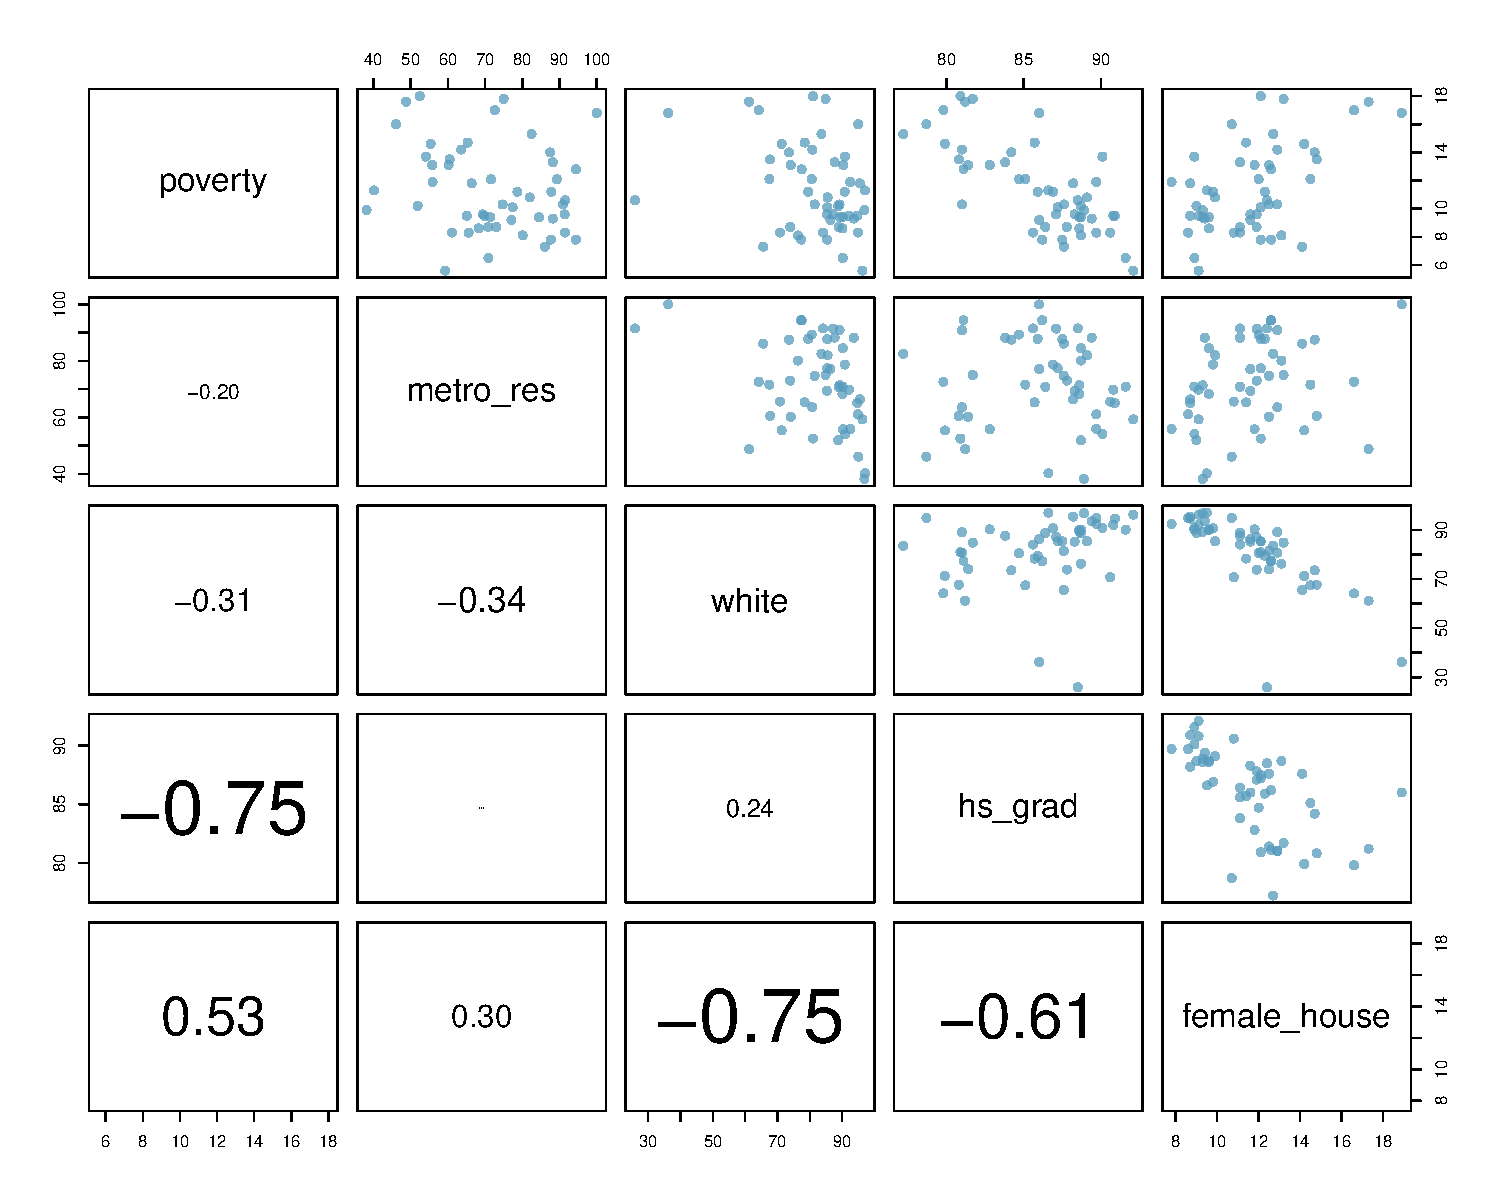
\includegraphics[width=0.9\textwidth]{9-1_intro_mlr/figures/poverty/poverty}
\end{center}

\end{frame}

%%%%%%%%%%%%%%%%%%%%%%%%%%%%%%%%%%%

\begin{frame}[fragile]
\frametitle{\% 女性世帯主を用いた貧困率の予測}

\vspace{-0.25cm}

\begin{center}
\begin{tabular}{rrrrr}
  \hline
 & Estimate & Std. Error & t value & Pr($>$$|$t$|$) \\
  \hline
(Intercept) & 3.31 & 1.90 & 1.74 & 0.09 \\
  female\_house & 0.69 & 0.16 & 4.32 & 0.00 \\
   \hline
\end{tabular}
\end{center}
\twocol{0.5}{0.4}
{
\begin{center}
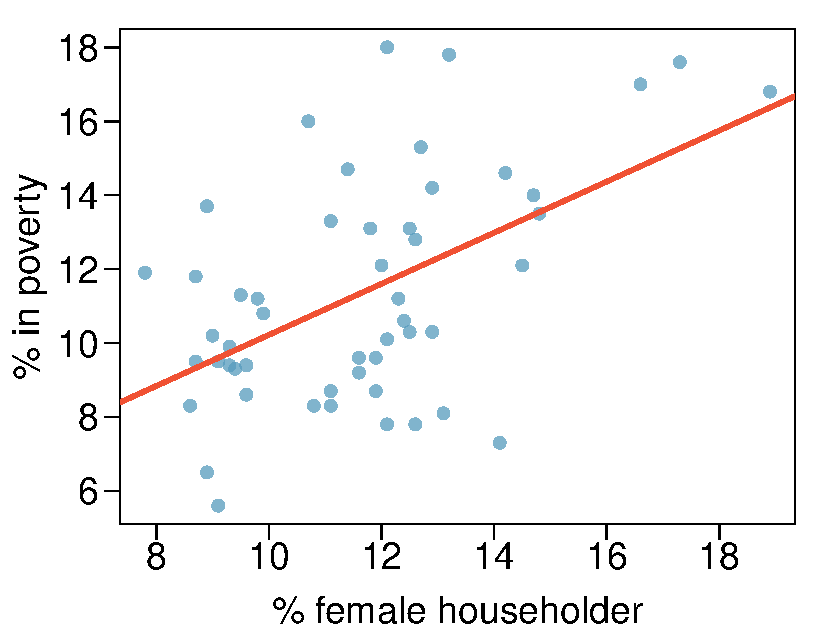
\includegraphics[width=\textwidth]{9-1_intro_mlr/figures/poverty/poverty_female_house}
\end{center}
}
{
\begin{align*}
R &= 0.53 \\
R^2 &= 0.53^2 = 0.28
\end{align*}
}

\end{frame}

%%%%%%%%%%%%%%%%%%%%%%%%%%%%%%%%%%%

\begin{frame}[fragile]
\frametitle{$R^2$ を改めて見る}

$R^2$ は3通りの方法で計算できる：

\begin{enumerate}

\item $x$ と $y$ の相関係数を2乗する {\small （これまでの計算方法）}

\item $y$ と $\hat{y}$ の相関係数を2乗する

\item 定義に基づいて計算する：

\[ R^2 = \frac{\text{$y$ の説明された変動}}{\text{$y$ の全変動}} \]

\end{enumerate}

\hl{分散分析（ANOVA）}を用いると、$y$ の説明された変動と全変動を計算できる。

\end{frame}


%%%%%%%%%%%%%%%%%%%%%%%%%%%%%%%%%%

\begin{frame}[fragile]
\frametitle{平方和}

\vspace{-0.5cm}

{\small
\begin{center}
\begin{tabular}{lrrrrr}
  \hline
 & Df & Sum Sq & Mean Sq & F value & Pr($>$F) \\
  \hline
female\_house & 1 & 132.57 & 132.57 & 18.68 & 0.00 \\
  Residuals & 49 & 347.68 & 7.10 &  &  \\
   \hline
Total & 50 & 480.25 \\
   \hline
\end{tabular}
\end{center}
}

\begin{changemargin}{-1cm}{-1cm}
\begin{eqnarray*}
\text{$y$ の平方和：} SS_{Total} &=& \sum(y - \bar{y})^2 = 480.25 \orange{ {\footnotesize ~$\rightarrow$ 全変動}} \\
\text{残差平方和：} SS_{Error} &=& \sum e_i^2 = 347.68 \orange{ { \footnotesize ~$\rightarrow$ 説明されていない変動}} \\
\text{$x$ の平方和：} SS_{Model} &=& SS_{Total} - SS_{Error} \orange{ {\footnotesize ~$\rightarrow$ 説明された変動}} \\
&=& 480.25 - 347.68 = 132.57
\end{eqnarray*}
\end{changemargin}

\[ R^2 = \frac{\text{説明された変動}}{\text{全変動}} = \frac{132.57}{480.25} = 0.28 \green{~$\checkmark$} \]

\end{frame}

%%%%%%%%%%%%%%%%%%%%%%%%%%%%%%%%%%

\begin{frame}
\frametitle{なぜ別の方法が必要か？}

\dq{相関係数の2乗として $R^2$ を計算する完全な方法があるのに、なぜ別のアプローチが必要なのか？}

\soln{\begin{itemize}
\item 単一予測変数の線形回帰では、同じ値を3通りで計算することはやりすぎに見えるかもしれない。
\item しかし、重線形回帰では $x$ が複数あるため、$x$ と $y$ の相関係数の2乗として $R^2$ を計算することができない。
\item 次に学ぶ \hl{自由度調整済み $R^2$} は説明された変動と説明されていない変動の比率という3番目のアプローチを必要とする。
\end{itemize}}

\end{frame}

%%%%%%%%%%%%%%%%%%%%%%%%%%%%%%%%%%

\begin{frame}
\frametitle{\% 女性世帯主 + \% 白人を用いた貧困率の予測}


\begin{center}
\begin{tabular}{rrrrr}
  \hline
\hl{線形モデル：}&  Estimate & Std. Error & t value & Pr($>$$|$t$|$) \\
  \hline
(Intercept) & -2.58 & 5.78 & -0.45 & 0.66 \\
  female\_house & 0.89 & 0.24 & 3.67 & 0.00 \\
  white & 0.04 & 0.04 & 1.08 & 0.29 \\
   \hline
\end{tabular}
\end{center}

\vspace{0.1cm}

\begin{center}
\begin{tabular}{lrrrrr}
  \hline
\hl{ANOVA：} & Df & Sum Sq & Mean Sq & F value & Pr($>$F) \\
  \hline
female\_house & 1 & 132.57 & 132.57 & 18.74 & 0.00 \\
  white & 1 & 8.21 & 8.21 & 1.16 & 0.29 \\
  Residuals & 48 & 339.47 & 7.07 &  &  \\
   \hline
Total & 50 &    480.25\\
   \hline
\end{tabular}
\end{center}

\[ R^2 = \frac{\text{説明された変動}}{\text{全変動}} = \frac{132.57 + 8.21}{480.25} = 0.29 \]

\end{frame}

%%%%%%%%%%%%%%%%%%%%%%%%%%%%%%%%%%%

\begin{frame}
\frametitle{}

\dq{変数 \var{white} をモデルに追加することで、\var{female\_house} が提供していなかった有益な情報が加わるか？}

\begin{center}
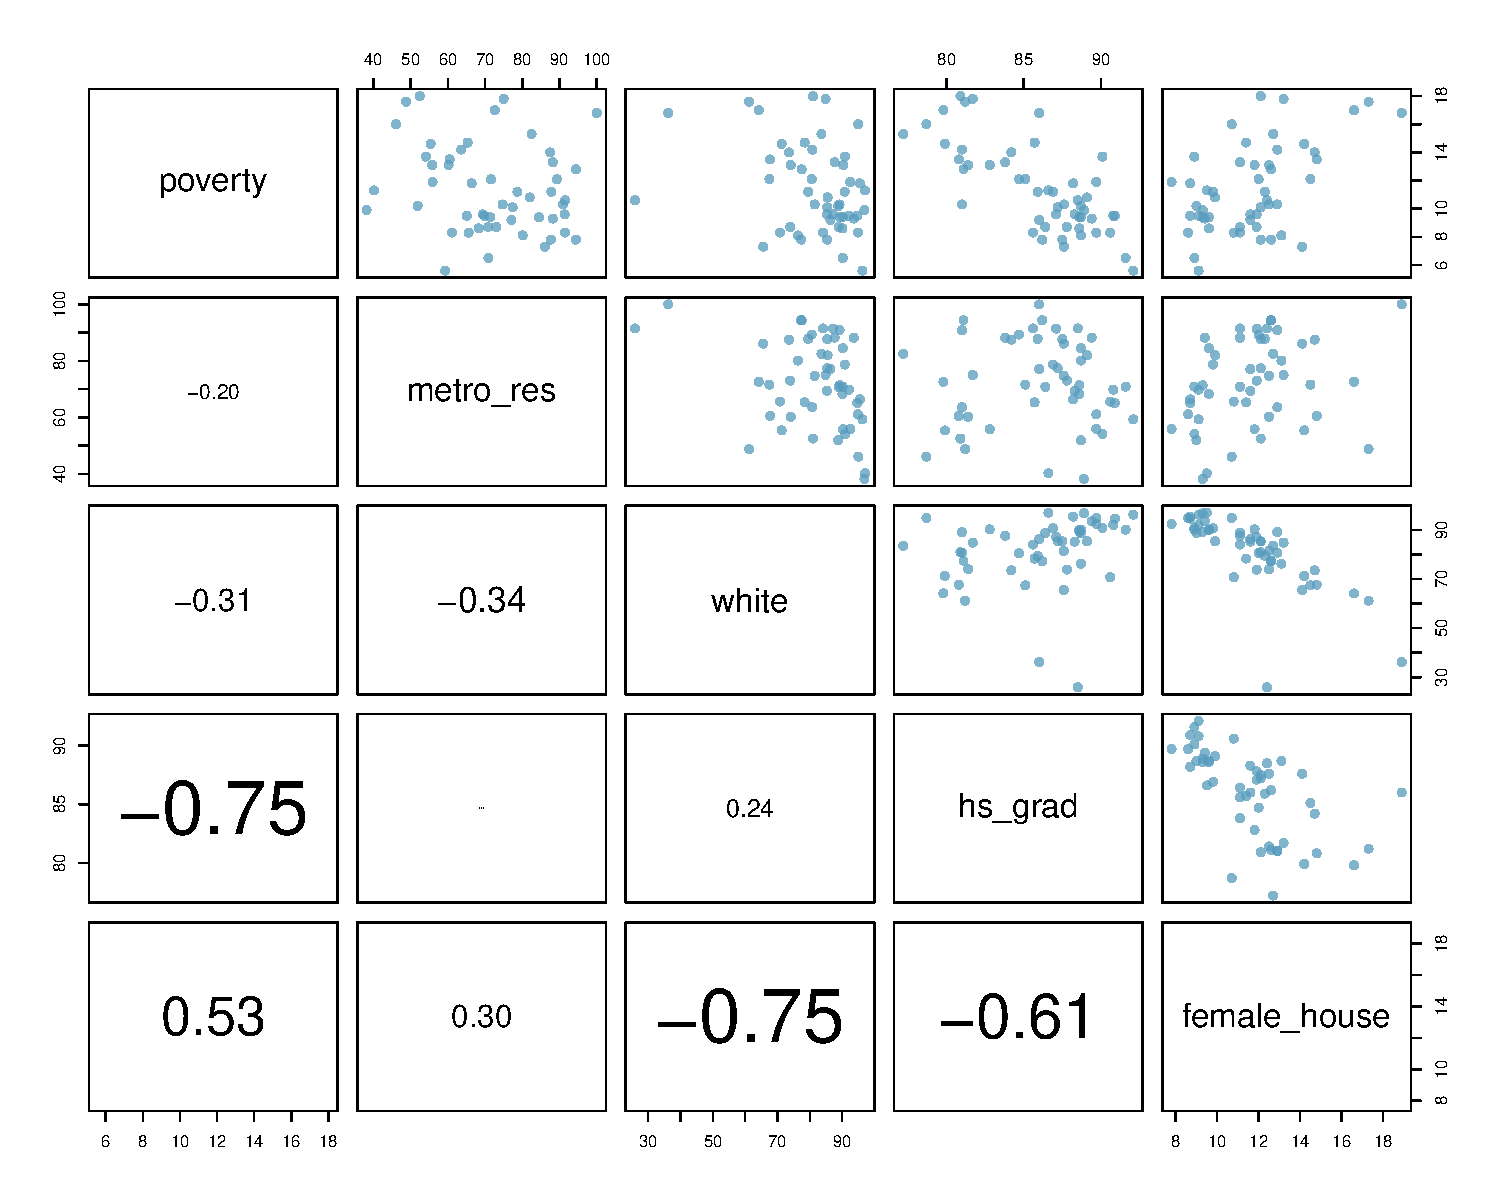
\includegraphics[width=0.8\textwidth]{9-1_intro_mlr/figures/poverty/poverty}
\end{center}

\end{frame}

%%%%%%%%%%%%%%%%%%%%%%%%%%%%%%%%%%%

\begin{frame}
\frametitle{説明変数間の多重共線性}

\hl{貧困率 vs. \% 女性世帯主}
\begin{center}
\begin{tabular}{rrrrr}
  \hline
 & Estimate & Std. Error & t value & Pr($>$$|$t$|$) \\
  \hline
(Intercept) & 3.31 & 1.90 & 1.74 & 0.09 \\
  female\_house & \orange{0.69} & 0.16 & 4.32 & 0.00 \\
   \hline
\end{tabular}
\end{center}

$\:$ \\

\hl{貧困率 vs. \% 女性世帯主 と \% 白人}
\begin{center}
\begin{tabular}{rrrrr}
  \hline
 & Estimate & Std. Error & t value & Pr($>$$|$t$|$) \\
  \hline
(Intercept) & -2.58 & 5.78 & -0.45 & 0.66 \\
  female\_house & \orange{0.89} & 0.24 & 3.67 & 0.00 \\
  white & 0.04 & 0.04 & 1.08 & 0.29 \\
   \hline
\end{tabular}
\end{center}

\end{frame}

%%%%%%%%%%%%%%%%%%%%%%%%%%%%%%%%%%%

\begin{frame}
\frametitle{説明変数間の多重共線性（続き）}

\begin{itemize}

\item 2つの予測変数が相関しているとき、それらは共線性があると言い、この\hl{多重共線性}はモデルの推定を複雑にする。\\
\Remember{予測変数は説明変数あるいは\underline{独立}変数とも呼ばれる。理想的には互いに独立であるべきである。}

\item 互いに関連した予測変数をモデルに加えることは好ましくない。そのような変数を追加しても、多くの場合何も得られないからである。代わりに、最もシンプルで優れたモデル、すなわち\hl{簡潔な（節約的な）}モデルを目指す。

\item 観測データから生じる多重共線性を完全に避けることは不可能だが、実験は通常、予測変数間の相関を防ぐように設計される。

\end{itemize}

\end{frame}

%%%%%%%%%%%%%%%%%%%%%%%%%%%%%%%%%%%

\begin{frame}[fragile]
\frametitle{$R^2$ vs. 自由度調整済み $R^2$}

\renewcommand\arraystretch{1.25}
\begin{center}
\begin{tabular}{l | c  c}
			& $R^2$	& 自由度調整済み $R^2$ \\
\hline
モデル1（単一予測変数）	& 0.28	& 0.26 \\
モデル2（重回帰）			& 0.29	& 0.26
\end{tabular}
\end{center}

\begin{itemize}

\item \underline{どんな}変数をモデルに加えても $R^2$ は増加する。

\item しかし、加えた変数が実際に新しい情報を提供しない場合や全く無関係な場合、自由度調整済み $R^2$ は増加しない。

\end{itemize}



\end{frame}

%%%%%%%%%%%%%%%%%%%%%%%%%%%%%%%%%%%

\begin{frame}
\frametitle{自由度調整済み $R^2$}

\formula{自由度調整済み $R^2$}
{\[ R^2_{adj} = 1 - \pr{ \frac{ SS_{Error} }{ SS_{Total} } \times \frac{n - 1}{n - p - 1} } \]
ここで $n$ はケース数、$p$ はモデル内の予測変数（説明変数）の数。
}

\begin{itemize}

\item $p$ が負になることはないため、$R^2_{adj}$ は常に $R^2$ より小さい。

\item $R^2_{adj}$ はモデルに含まれる予測変数の数に対してペナルティを課す。

\item したがって、$R^2_{adj}$ が高いモデルをより好ましいモデルとして選ぶ。

\end{itemize}

\end{frame}

%%%%%%%%%%%%%%%%%%%%%%%%%%%%%%%%%%%

\begin{frame}
\frametitle{自由度調整済み $R^2$ の計算}

\begin{center}
\begin{tabular}{lrrrrr}
  \hline
\hl{ANOVA：} & Df & Sum Sq & Mean Sq & F value & Pr($>$F) \\
  \hline
female\_house & 1 & 132.57 & 132.57 & 18.74 & 0.0001 \\
  white & 1 & 8.21 & 8.21 & 1.16 & 0.2868 \\
  Residuals & 48 & 339.47 & 7.07 &  &  \\
   \hline
Total & 50 &    480.25\\
   \hline
\end{tabular}
\end{center}

\begin{eqnarray*}
R^2_{adj} &=& 1 - \pr{ \frac{ SS_{Error} }{ SS_{Total} } \times \frac{n - 1}{n - p - 1} } \\
&=& 1 - \pr{ \frac{ 339.47 }{ 480.25 } \times \frac{51 - 1}{51 - 2 - 1} }   \\
&=& 1- \pr{ \frac{ 339.47 }{ 480.25 } \times \frac{50}{48} } \\
&=& 1 -  0.74 \\
&=& 0.26
\end{eqnarray*}

\end{frame}
